\documentclass{beamer}
\usetheme{metropolis}
%\usepackage[backend=biber]{biblatex}
%\usepackage{booktabs} 
\usepackage{url}
\def\UrlBreaks{\do\/\do-}
\usepackage{amsfonts, amsmath, lmodern}
\usefonttheme{serif}
\usepackage{algorithm}
\usepackage{algorithmic}
\usepackage{amssymb}


%plots
\usepackage{tikz}
\usepackage{pgfplots}
\usepackage{pgfplotstable}
\pgfplotsset{compat=newest}
\usepackage{subcaption}
\usepackage{csvsimple}
%bibliography numbers
\setbeamertemplate{bibliography item}{\insertbiblabel}

\graphicspath{{./pictures}}
\setbeameroption{show notes} % comment out for the real presentation

\title{Fast Search of the Optimal Contraction Sequence in Tensor Networks}

\author{Max Koch, Christian Ortlepp}


\institute{Friedrich-Schiller-Universität Jena}

\date{20. Januar 2023}

\newcommand{\Tau}{\mathcal{T}}




\begin{document}

\begin{frame}
	\titlepage
\end{frame}

\begin{frame}{Gliederung}
	\tableofcontents
\end{frame}

\section{Einführung und Zielsetzung}
\begin{frame}{Einführung}
	\begin{itemize}
		\item viele Anwendungen: Quantenphysik, Machine Learning, Entwurf von elektrischen Schaltungen
		\item Reihenfolge der Kontraktionen beeinflusst sowohl Speicher als auch Rechenaufwand
		\item Problem: das Finden der optimalen Reihenfolge ist NP-hart
		\item[$\Rightarrow$] Heuristiken  
	\end{itemize}
\end{frame}

\begin{frame}{Zielsetung}
	\begin{itemize}
		\item Entwurf eines universalen Algorithmus \begin{itemize}
			\item effiziente Datenstruktur für die Suche
			\item für alle Netzwerktopologien anwendbar
			\item Multithreading für bessere reale Performanz
		\end{itemize}   
		\item[$\Rightarrow$] Benchmarks
	\end{itemize}
\end{frame}

\section{Tensor-Kontraktionen}
\subsection{Allgemeines}

\begin{frame}{Begriffseinführungen}
	\begin{columns}
		\begin{column}{0.5\textwidth}
			\begin{itemize}
				\item $\tau$: Tensor
				\item $\Tau_I$: Ergebnis-Tensor aus der Kontraktion der Tensoren $I$
				\item $FO_{\Tau_I}$: Free Orders von $\Tau_I$
				\item $SO_{\Tau_I}$: Sharing Orders von $\Tau_I$
			\end{itemize}
		\end{column}
		\begin{column}{0.5\textwidth}
			\begin{itemize}
				\item $SE_{\Tau_I}$: Storage Expense von $\Tau_I$
				\item $CE_{\Tau_I}$: Storage Expense von $\Tau_I$
				\item $MS$: Maximale $SE$ einer Kontraktion 
				\item $MC$: Maximale $CE$ einer Kontraktion 
			\end{itemize}
		\end{column}
	\end{columns}
\end{frame}
\note[itemize]{
	\item CE: Anzahl der Multiplikationen
}

\begin{frame}{Begriffseinführungen}
	\begin{columns}
		\begin{column}{0.5\textwidth}
			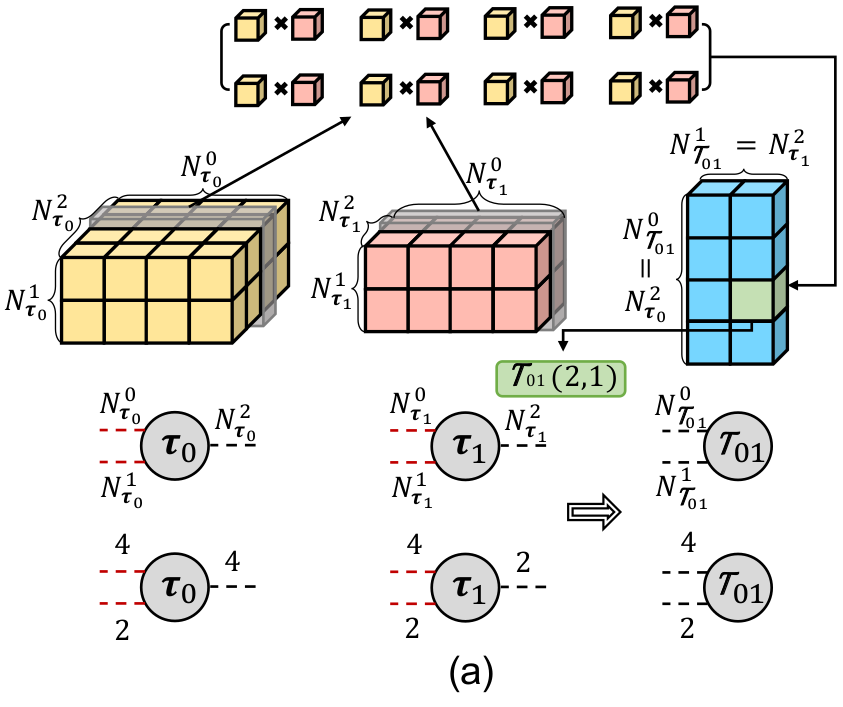
\includegraphics[scale=.2]{figure-2-a}
		\end{column}
		\begin{column}{0.5\textwidth}
			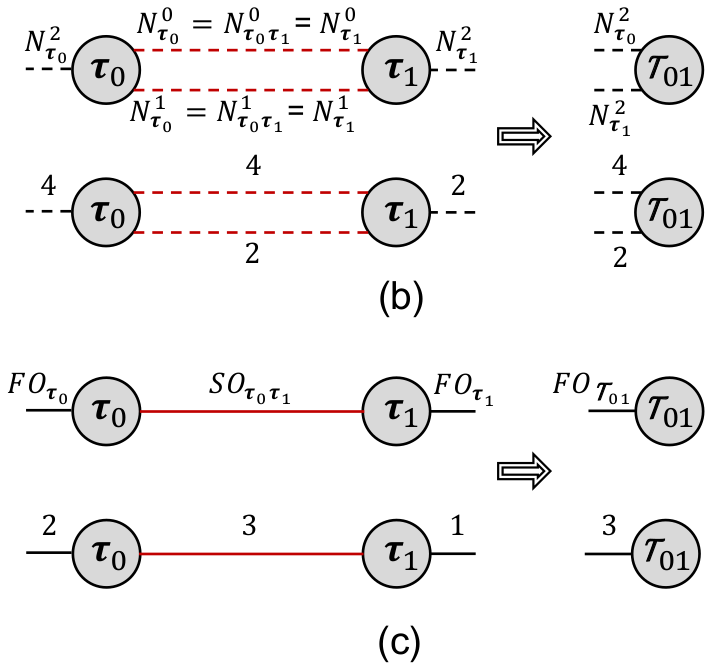
\includegraphics[scale=.2]{figure-2-b}
		\end{column}
	\end{columns}
\end{frame}
\note[itemize]{
	\item a:
	\item Graph-Notation: Kanten=Dimensionen (Order), Knoten=Tensoren
	\item b:
	\item Kanten zwischen Knoten "Sharing Orders", sonst "Free Orders"
	\item Nach der Kontraktion bleiben nur Free Orders übrig
	\item c:
	\item Kantengewicht: $\log_2$ der Order (Vereinfachung der Rechnung)
}

\begin{frame}{Formeln}
	\begin{equation}
		FO_{\Tau_I}=\sum\limits_m \log_k N_{\Tau_I}^m, N_{\Tau_I}^m \in \text{ free orders of } \Tau_I 
	\end{equation}
	\begin{equation}
		SO_{\Tau_I\Tau_J}=\sum\limits_m \log_k N_{\Tau_I\Tau_J}^m 
	\end{equation}
	\begin{equation}
		S_{\Tau_I}=FO_{\Tau_I}+\sum\limits_J SO_{\Tau_I\Tau_J}, \text{ where } J\notin I
	\end{equation}
	\begin{equation}
		SE_{\Tau_I\Tau_J}=S_{\Tau_{IJ}}=S_{\Tau_I}+S_{\Tau_J}-2SO_{\Tau_I\Tau_J}
	\end{equation}
	\begin{equation}
		CE_{\Tau_I\Tau_J}=S_{\Tau_I}+S_{\Tau_J}-SO_{\Tau_I\Tau_J}=S_{\Tau_{IJ}}+SO_{\Tau_I\Tau_J}
	\end{equation}
\end{frame}

\begin{frame}{Kontraktion}
	\begin{columns}
		\begin{column}{0.5\textwidth}
			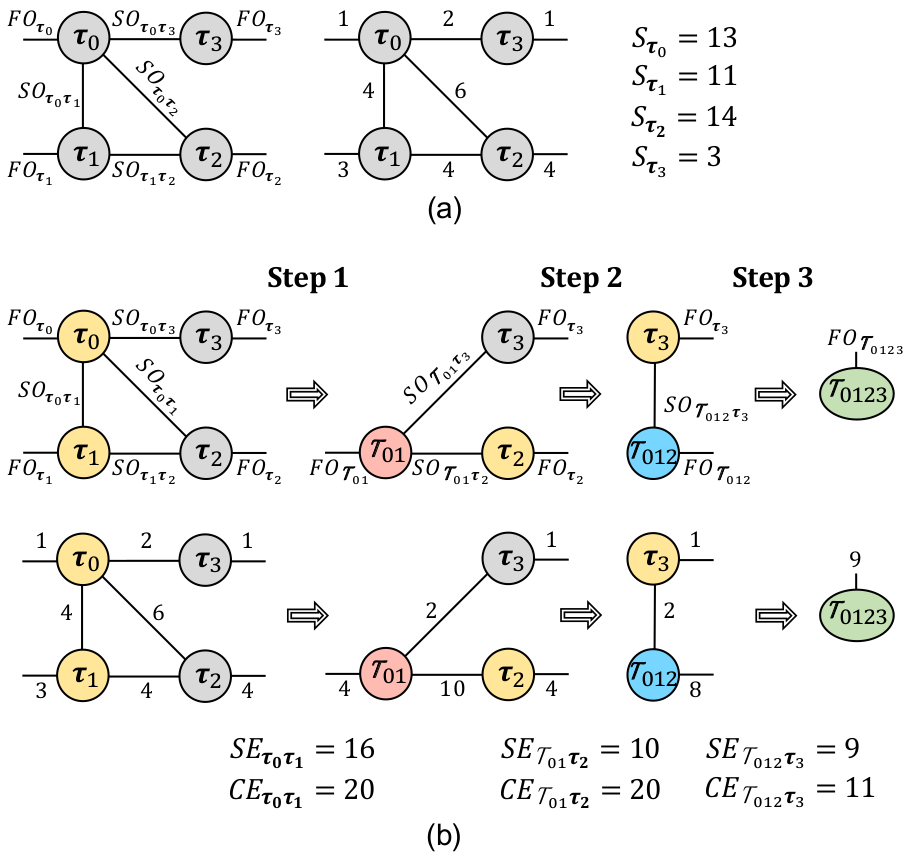
\includegraphics[scale=.17]{figure-3-a}
			$(b) sq=(((\tau_0\tau_1)\tau_2)\tau_3)$
		\end{column}
		\begin{column}{0.5\textwidth}
			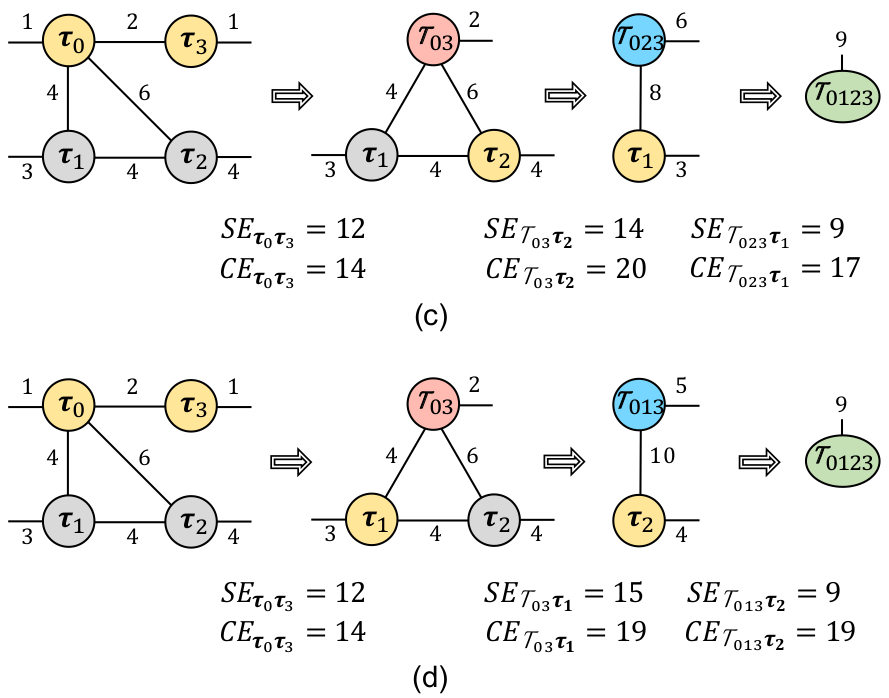
\includegraphics[scale=.17]{figure-3-b}
		\end{column}
	\end{columns}
\end{frame}
\note[itemize]{
	\item bei K Tensoren immer K-1 Kontraktionsschritte
	\item verschiedene Kontraktionsreihenfolgen
	\item bei jedem Schritt wird eine sharing order eliminiert
}

\section{Adjazenzmatrix-basierte Kontraktionssuche}

\subsection{Vanilla Search}
\begin{frame}{Sharing Order Calculation}
	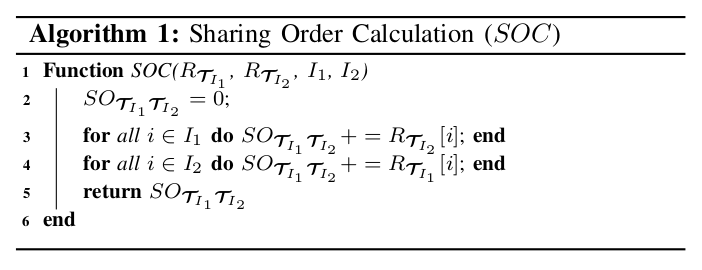
\includegraphics[scale=0.4]{algorithm-1}
\end{frame}
\note[itemize]{
	\item WICHTIG: ab jetzt arbeiten wir auf den Adjazenzmatrizen und nicht auf den tensoren selbst
	\item input:
	\item zwei zeilen-vektoren  der  Matrizen zu kontrahierenden Tensoren
	\item die Menge der Tensoren, aus welchen die inputs (durch vorherige Kontraktionen) entstanden sind
}
\begin{frame}{Vanilla Search - Teil 1}
	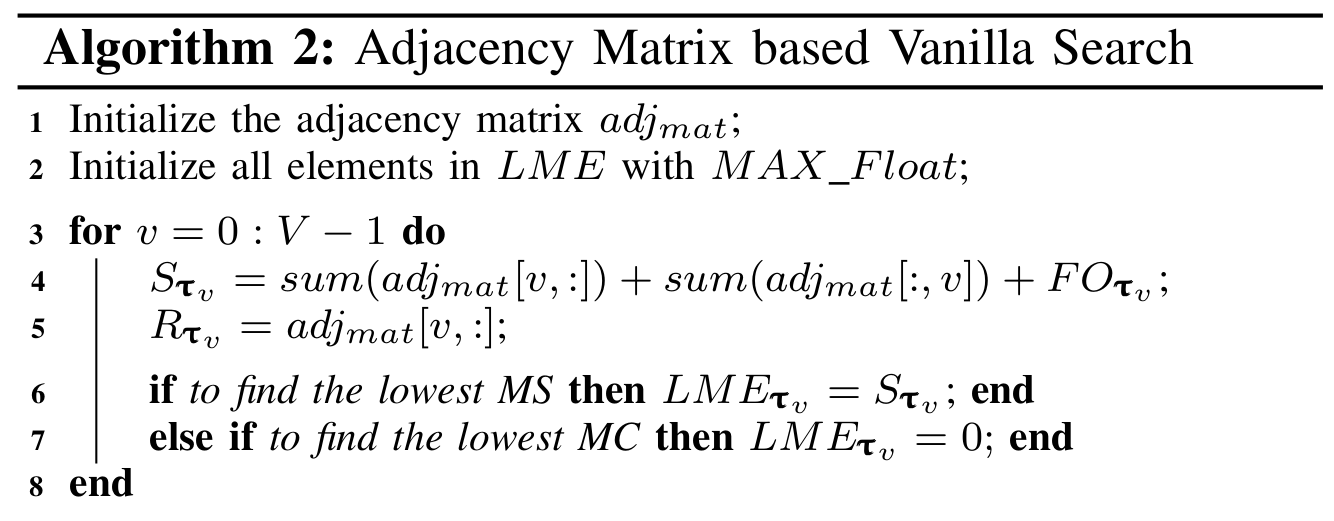
\includegraphics[scale=0.2]{algorithm-2-a}
\end{frame}
\note[itemize]{
	\item 1-2: initialisiere Adjazenzmatrix und Lowest Maximum Expense für alle tensoren
	\item 3: iteriere über alle Tensoren im Netzwerk
	\item 4: speichere die Größe des Tensors (Data Size)
	\item 5: speichere Zeilenvektor aus Adjazenzmatrix
	\item 6-7: Je nach modus (compute/storage) wird LME unterschiedlich initialisiert
}
\begin{frame}{Vanilla Search - Teil 2}
	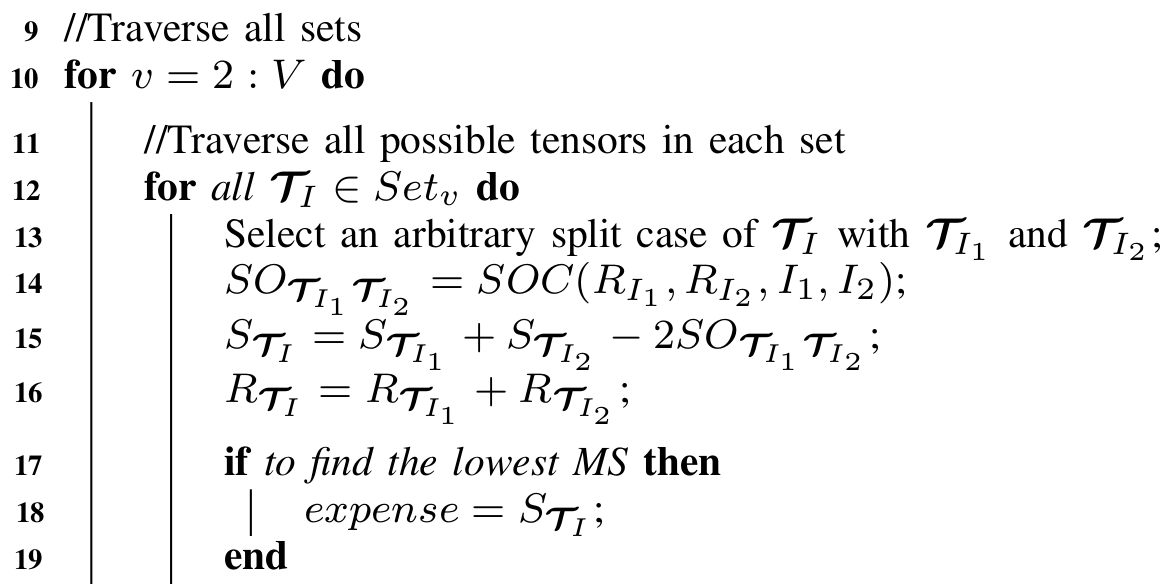
\includegraphics[scale=0.25]{algorithm-2-b}
\end{frame}
\note[itemize]{
	\item 10: iteriere über möglichen Kontraktions-Größen
	\item 12: iteriere über alle Tensoren im Set. Größe des aktuellen Tensor: $S_{T_I}$, Repräsentation dieses Tensors als Zeilenvektor: $R_{T_I}$
	\item 13: wähle beliebig einen split-case des aktuellen Tensors $T_I$
	\item 15-16: berechne den Zeilenvektor und Data Size von $T_I$
	\item 17: Falls neues MS gefunden wurde wird dies gespeichert
	\item Generell: initialisiert nur variablen, die tatsächliche Berechnung geschieht in Teil 3
}
\begin{frame}{Vanilla Search - Teil 3}
	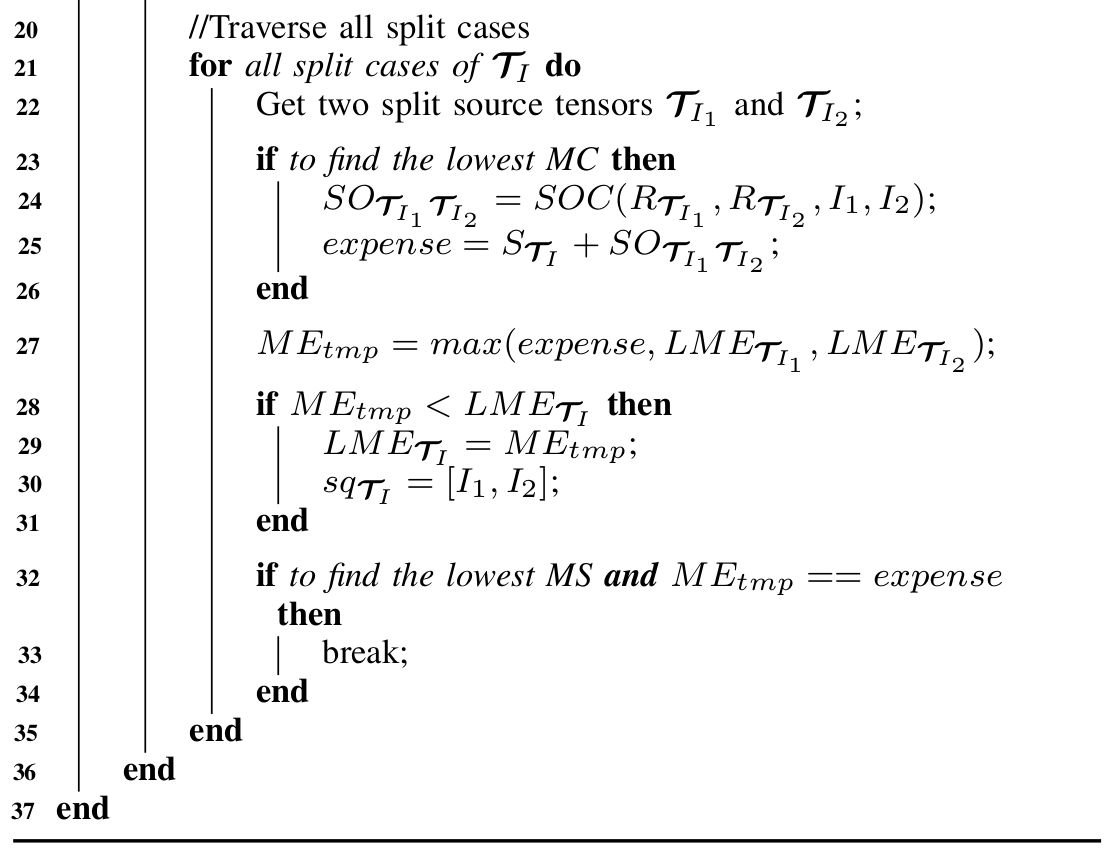
\includegraphics[scale=0.25]{algorithm-2-c}
\end{frame}
\note[itemize]{
	\item WICHTIG: immernoch innerhalb der vorherigen beiden Schleifen
	\item 21: Iteriere über jeden split case von $T_I$
}


\subsection{Outer Product Pruning}
\begin{frame}{Pruning - Einührung}
	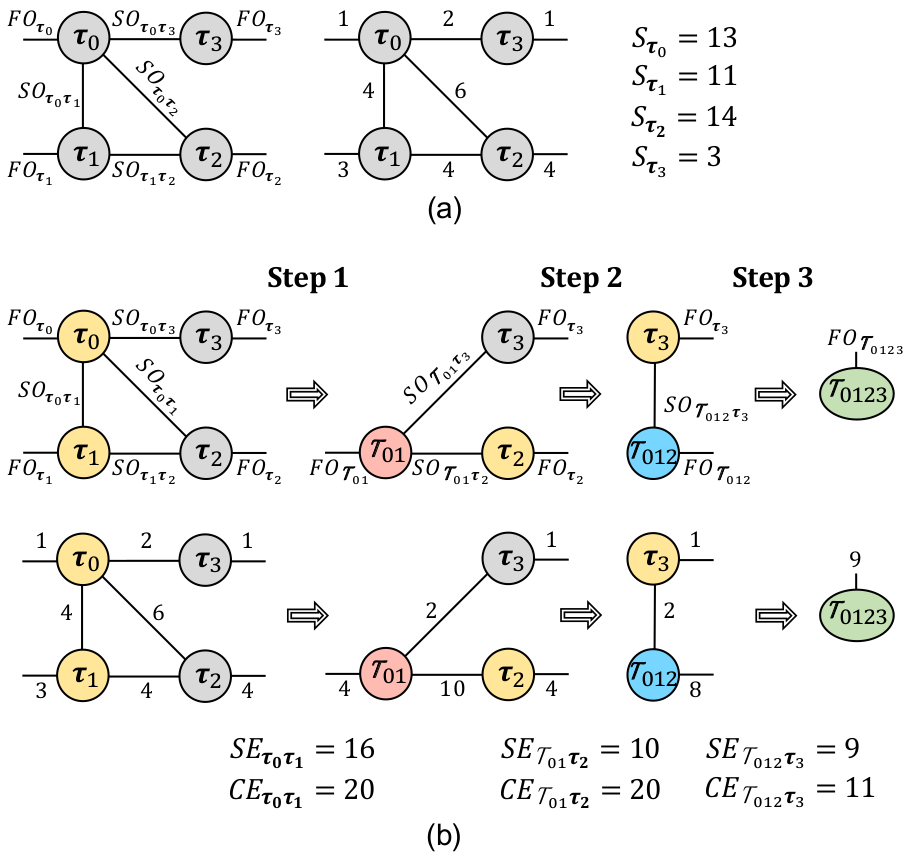
\includegraphics[scale=0.2]{figure-3-a}
\end{frame}
\note[itemize]{
	\item outer product: multiplikation von Tensoren ohne sharing Orders (siehe $\tau_2, \tau_3$)
	\item es ist bewiesen dass die beste Kontraktion (kleinste MS / MC) immer ohne outer - products auskommt
	\item[$\Rightarrow$] Outer products können bei Kontraktionen ausgeschlossen werden
	\item Wenn es im Netzwerk "Subnetzwerke" gibt, welche untereinander keine sharing orders teilen, kann in den subnetzwerken unabhängig voneinander nach der optimalen sequenz gesucht werden
}
\begin{frame}{Pruning - Einführung}
	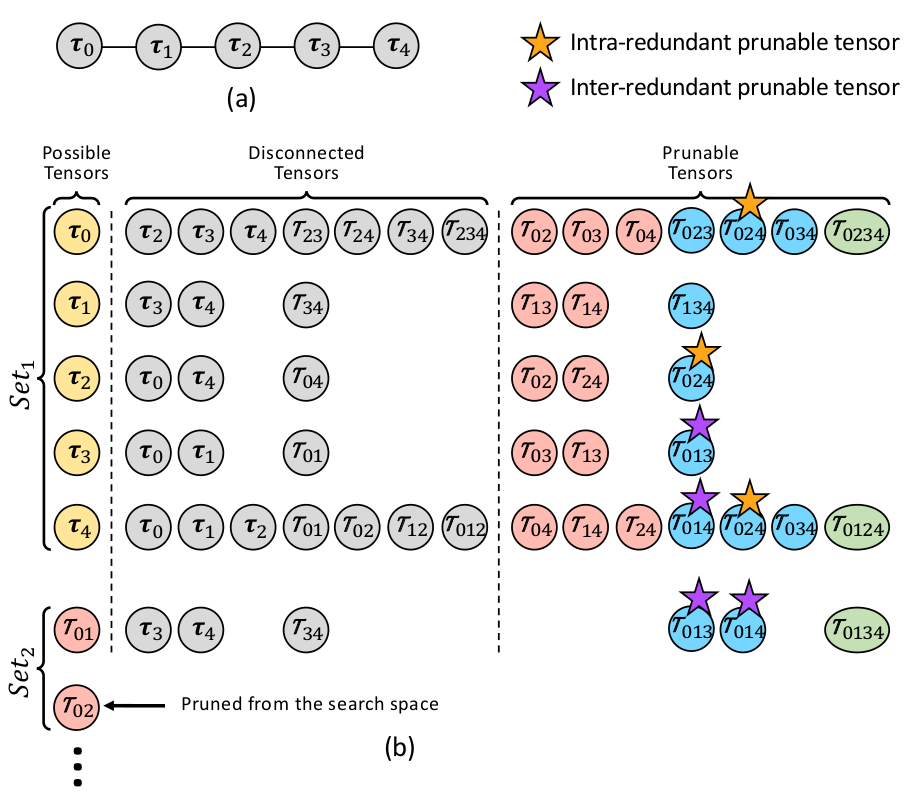
\includegraphics[scale=0.25]{figure-6}
\end{frame}
\note[itemize]{
	\item Intra-redundant: innerhalb eines Set
	\item Inter-redundant: zwischen verschiedenen Sets
}

\begin{frame}{Pruning - Adjazenzmatrix}
	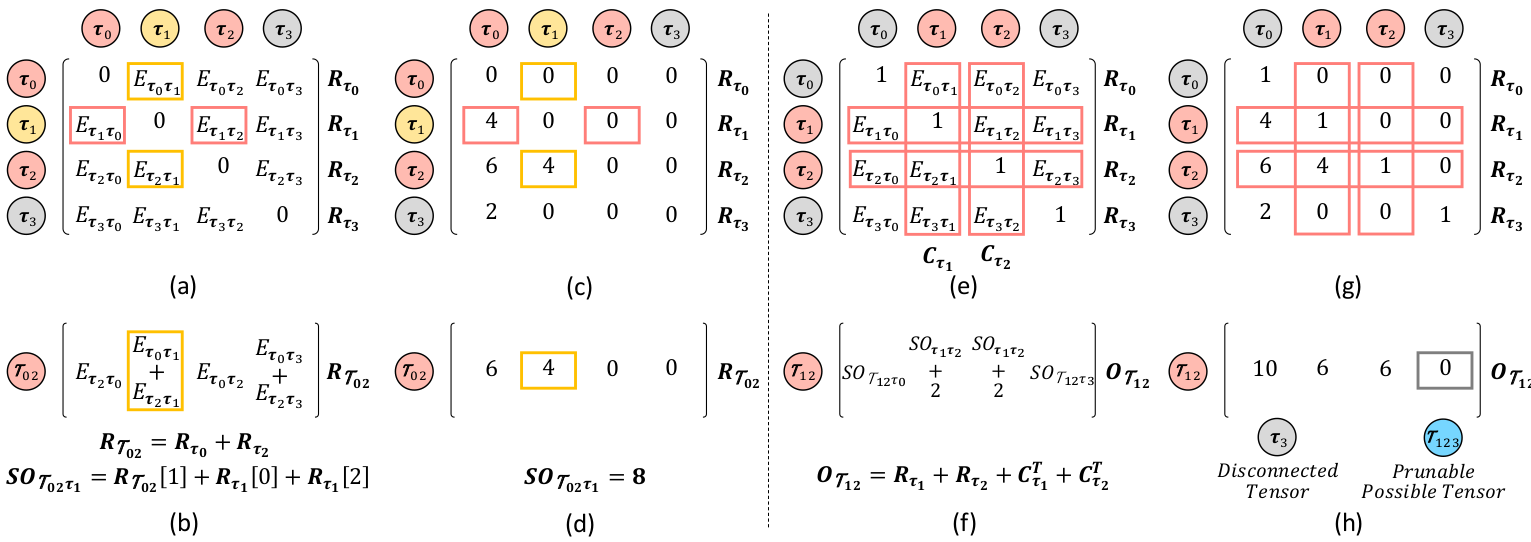
\includegraphics[scale=0.2]{figure-5}
\end{frame}
\note[itemize]{
	\item TODO Figure 5 Adjazenzmatrix Struktur
}

\begin{frame}{Pruning - Algorithmus}
	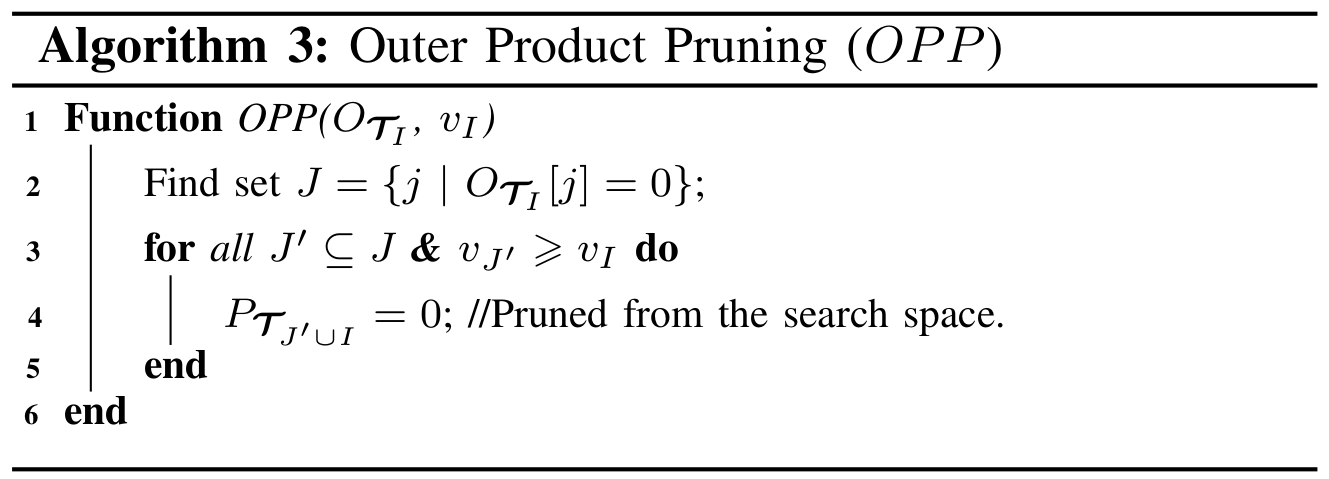
\includegraphics[scale=0.25]{algorithm-3}
\end{frame}
\note[itemize]{
	\item someNote
}
\section{Ergebnisse}

\begin{frame}{Benchmarks}
	\begin{itemize}
		\item getestet auf verschiedenen Topologien (Kette, Baum, Radial und Gitter)
		\item Anzahl zusätzlicher Kanten variabel
	\end{itemize}
\end{frame}
\note[itemize]{
	\item 
}
\begin{frame}{Suche - Baseline}
	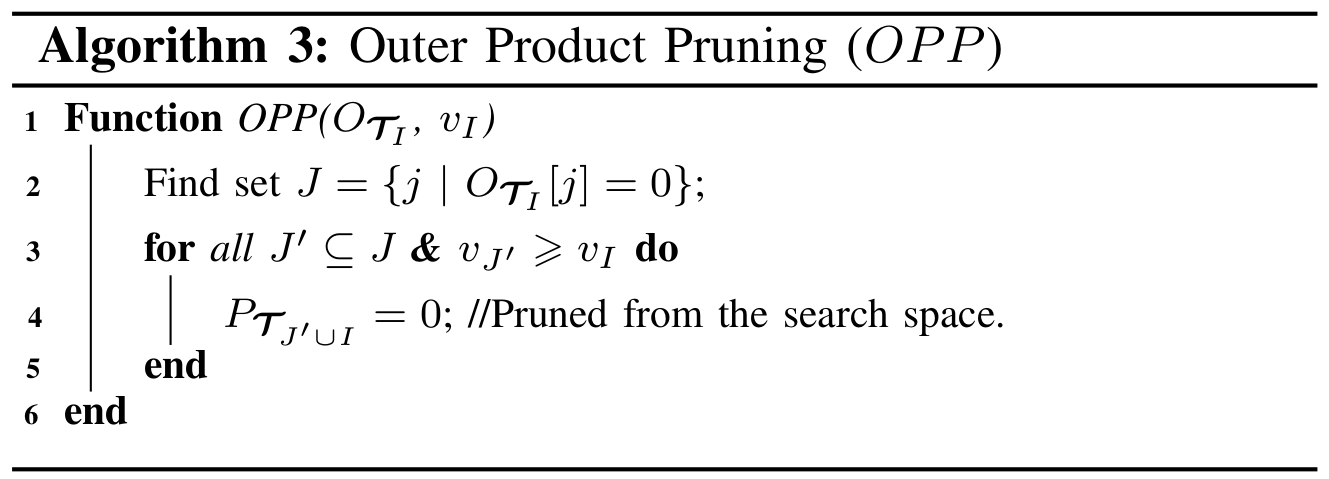
\includegraphics[scale=0.25]{table-3}
\end{frame}
\note[itemize]{
	\item 19 Tensoren, keine zusätzlichen Kanten
	\item pruning verbessert Suchzeiten, bei MC effektiver als bei MS
	\item Kette ist besser als Baum ist besser als Radial
}
\begin{frame}{Suche - Kette, Baum, Radial}
	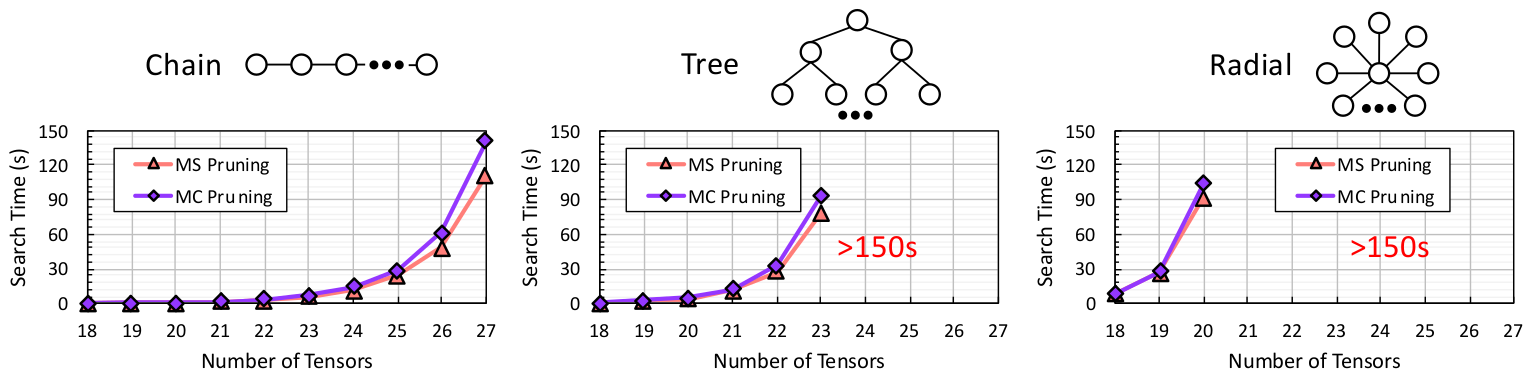
\includegraphics[scale=0.2]{figure-9}
	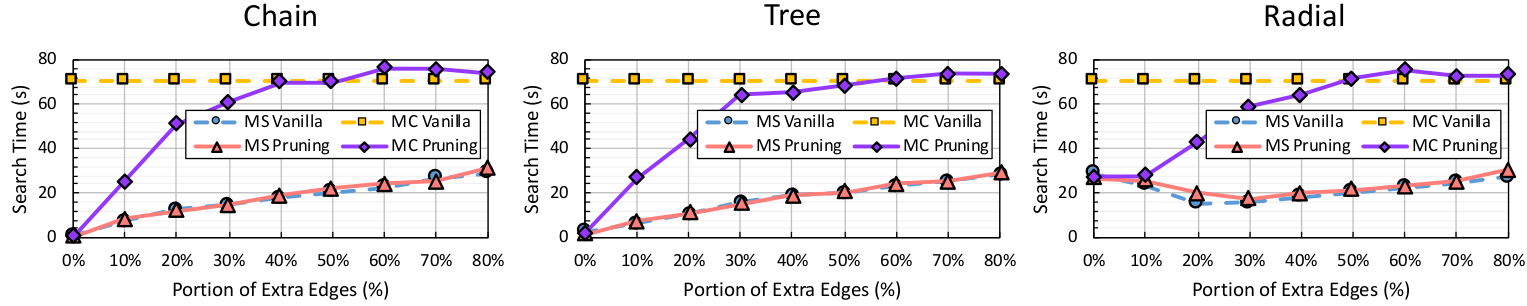
\includegraphics[scale=0.2]{figure-10}
\end{frame}
\note[itemize]{
	\item fig 9: Vergleich MS vs MC auf verschiedenen Topologien
	\item bei Baum und Radial abgheschnitten da zu lange suchzeiten (> 150s)
	\item Kette: hat die meisten prunable tensors, deswegen ist es dort am effektivsten
	\item 
}
\begin{frame}{Suche - Gitter}
	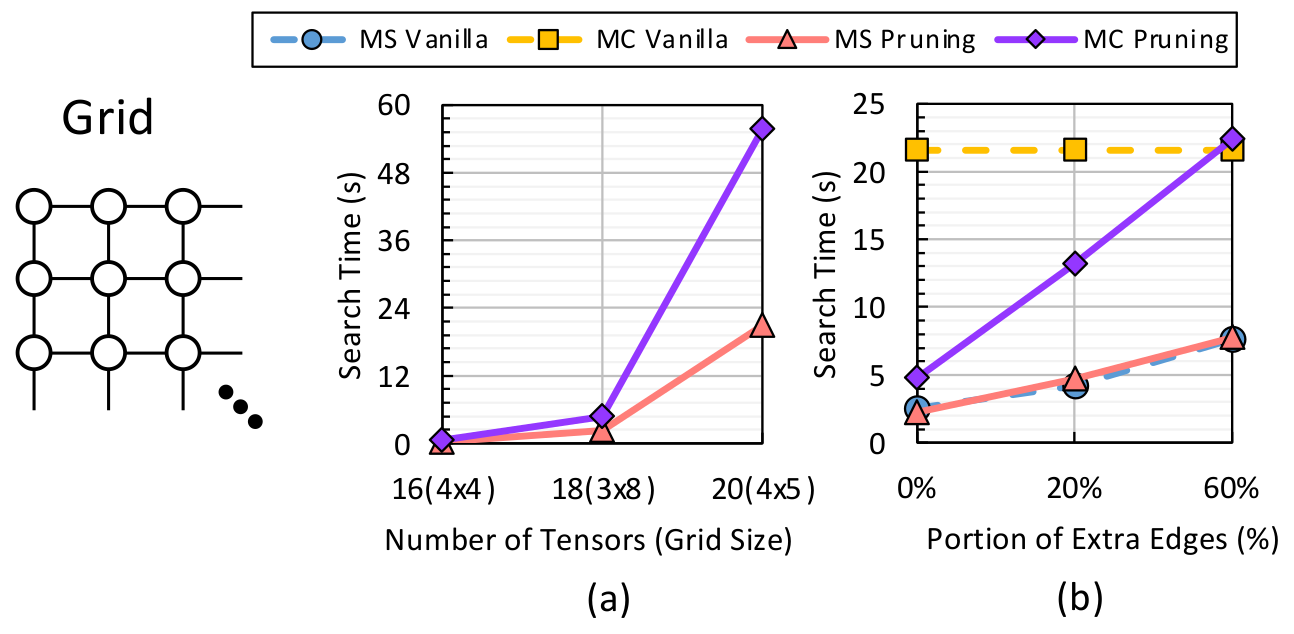
\includegraphics[scale=0.2]{figure-11}
\end{frame}
\note[itemize]{
	\item
}


\begin{frame}[allowframebreaks]{Bibliography}
	\bibliography{../bibliography/bibliography.bib}
	\bibliographystyle{splncs04}
	\nocite{*}
\end{frame}

\end{document}
